\documentclass{article}

\usepackage{fancyhdr}
\usepackage{extramarks}
\usepackage{amsmath}
\usepackage{amsthm}
\usepackage{amsfonts}
\usepackage{tikz}
\usepackage[plain]{algorithm}
\usepackage{algpseudocode}
\usepackage{enumerate}
\usepackage{amssymb}
\usepackage[margin=1in]{geometry}

\newcommand{\st}{~\mid~}
\newcommand{\ind}{$~~~$}
\usepackage{xcolor}

\graphicspath{ {./../images} }

\usetikzlibrary{automata,positioning}

%
% Basic Document Settings
%

\topmargin=-0.45in
\evensidemargin=0in
\oddsidemargin=0in
\textwidth=6.5in
\textheight=9.0in
\headsep=0.25in

\linespread{1.1}

\pagestyle{fancy}
\lhead{\hmwkAuthorName}
\chead{\hmwkClass:\ \hmwkTitle}
\rhead{\firstxmark}
\lfoot{\lastxmark}
\cfoot{\thepage}

\renewcommand\headrulewidth{0.4pt}
\renewcommand\footrulewidth{0.4pt}

\setlength\parindent{0pt}
\setlength{\parskip}{5pt}

%
% Create Problem Sections
%

\newcommand{\enterProblemHeader}[1]{
    \nobreak\extramarks{}{Problem \arabic{#1} continued on next page\ldots}\nobreak{}
    \nobreak\extramarks{Problem \arabic{#1} (continued)}{Problem \arabic{#1} continued on next page\ldots}\nobreak{}
}

\newcommand{\exitProblemHeader}[1]{
    \nobreak\extramarks{Problem \arabic{#1} (continued)}{Problem \arabic{#1} continued on next page\ldots}\nobreak{}
    \stepcounter{#1}
    \nobreak\extramarks{Problem \arabic{#1}}{}\nobreak{}
}

\setcounter{secnumdepth}{0}
\newcounter{partCounter}
\newcounter{homeworkProblemCounter}
\setcounter{homeworkProblemCounter}{1}
\nobreak\extramarks{Problem \arabic{homeworkProblemCounter}}{}\nobreak{}

%
% Homework Problem Environment
%
% This environment takes an optional argument. When given, it will adjust the
% problem counter. This is useful for when the problems given for your
% assignment aren't sequential. See the last 3 problems of this template for an
% example.
%
\newenvironment{homeworkProblem}[1][-1]{
    \ifnum#1>0
        \setcounter{homeworkProblemCounter}{#1}
    \fi
    \section{Problem \arabic{homeworkProblemCounter}}
    \setcounter{partCounter}{1}
    \enterProblemHeader{homeworkProblemCounter}
}{
    \exitProblemHeader{homeworkProblemCounter}
}

%
% Homework Details
%   - Title
%   - Due date
%   - Class
%   - Section/Time
%   - Instructor
%   - Author
%

\newcommand{\hmwkTitle}{Homework\ \#1}
\newcommand{\hmwkDueDate}{Apr 10, 2024}
\newcommand{\hmwkClass}{CSE 101}
\newcommand{\hmwkClassInstructor}{Professor Jones}
\newcommand{\hmwkAuthorName}{\textbf{Ray Tsai}}
\newcommand{\hmwkPID}{A16848188}

%
% Title Page
%

\title{
    \vspace{2in}
    \textmd{\textbf{\hmwkClass:\ \hmwkTitle}}\\
    \normalsize\vspace{0.1in}\small{Due\ on\ \hmwkDueDate\ at 23:59pm}\\
    \vspace{0.1in}\large{\textit{\hmwkClassInstructor}} \\
    \vspace{3in}
}

\author{
  \hmwkAuthorName \\
  \vspace{0.1in}\small\hmwkPID
}
\date{}

\renewcommand{\part}[1]{\textbf{\large Part \Alph{partCounter}}\stepcounter{partCounter}\\}

%
% Various Helper Commands
%

% Useful for algorithms
\newcommand{\alg}[1]{\textsc{\bfseries \footnotesize #1}}

% For derivatives
\newcommand{\deriv}[1]{\frac{\mathrm{d}}{\mathrm{d}x} (#1)}

% For partial derivatives
\newcommand{\pderiv}[2]{\frac{\partial}{\partial #1} (#2)}

% Integral dx
\newcommand{\dx}{\mathrm{d}x}

% Probability commands: Expectation, Variance, Covariance, Bias
\newcommand{\Var}{\mathrm{Var}}
\newcommand{\Cov}{\mathrm{Cov}}
\newcommand{\Bias}{\mathrm{Bias}}
\newcommand*{\Z}{\mathbb{Z}}
\newcommand*{\Q}{\mathbb{Q}}
\newcommand*{\R}{\mathbb{R}}
\newcommand*{\C}{\mathbb{C}}
\newcommand*{\N}{\mathbb{N}}
\newcommand*{\prob}{\mathds{P}}
\newcommand*{\E}{\mathds{E}}

\begin{document}

\maketitle

\pagebreak

\begin{homeworkProblem}
  Let $T$ be defined by the recurrence relation:

  \[
    T(0) = 1~,T(1) = 4~~~~~~~ T(n) = T(n-1) + 2T(n-2) + (3)(2^{n-1})~~for~~all~~n\geq 2
  \]

  \begin{enumerate}[(a)]
  \item Prove that $T(n)=\Omega(2^n)$ using induction.
  \begin{proof}
    Pick $n_0 = 0$. We show that $T(n) \geq 2^n$ for all $n \geq n_0$ by induction on $n$. The base
    cases are trivial, as $T(0) = 1 \geq 2^0$ and $T(1) = 4 \geq 2^1$. Suppose $n \geq 2$. By
    induction, 
    \begin{align*}
      T(n) 
      &= T(n-1) + 2T(n-2) + 3 \cdot 2^{n-1} \\
      &\geq 2^{n - 1} + 2 \cdot 2^{n - 2} + 3 \cdot 2^{n-1} = \frac{5}{2} \cdot 2^{n} > 2^{n},
    \end{align*}
    and we are done.
  \end{proof}

  \item Prove that $T(n) = O(n2^n)$ using induction.
  \begin{proof}
    Pick $c = 2$ and $n_0 = 1$. We show that $T(n) \leq cn2^n$ for $n \geq n_0$ by induction on $n$.
    Since $T(1) = 4 \leq c \cdot 2 = 4$ and $T(2) = 12 \leq c \cdot 2 \cdot 2^{2} = 16$, the base
    case is done. Suppose $n > 2$. By induction,
    \begin{align*}
      T(n) 
      &= T(n-1) + 2T(n-2) + 3 \cdot 2^{n-1} \\
      &\leq c(n-1)2^{n - 1} + 2c(n-2)2^{n - 2} + 3 \cdot 2^{n-1} \\
      &= (4n - 3)2^{n - 1} = 2\left(n - \frac{3}{4}\right)2^n \leq c \cdot n2^n,
    \end{align*}
    and we are done.
  \end{proof}
  \end{enumerate}
\end{homeworkProblem}

\newpage

\begin{homeworkProblem}
  Let $B(n)$ be the $n$th \emph{Complete Balanced Bipartite Graph} on $2n$ vertices. $B(n)$ has $2n$
  vertices $n$ on each side. One side has vertices labeled $a_1,\dots,a_n$ and the other side has
  vertices labeled $b_1,\dots,b_n$. There is an edge connecting $a_i$ and $b_j$ for all $1\leq
  i,j\leq n$

  Below is the graph of $B(3):$
  \begin{center}
    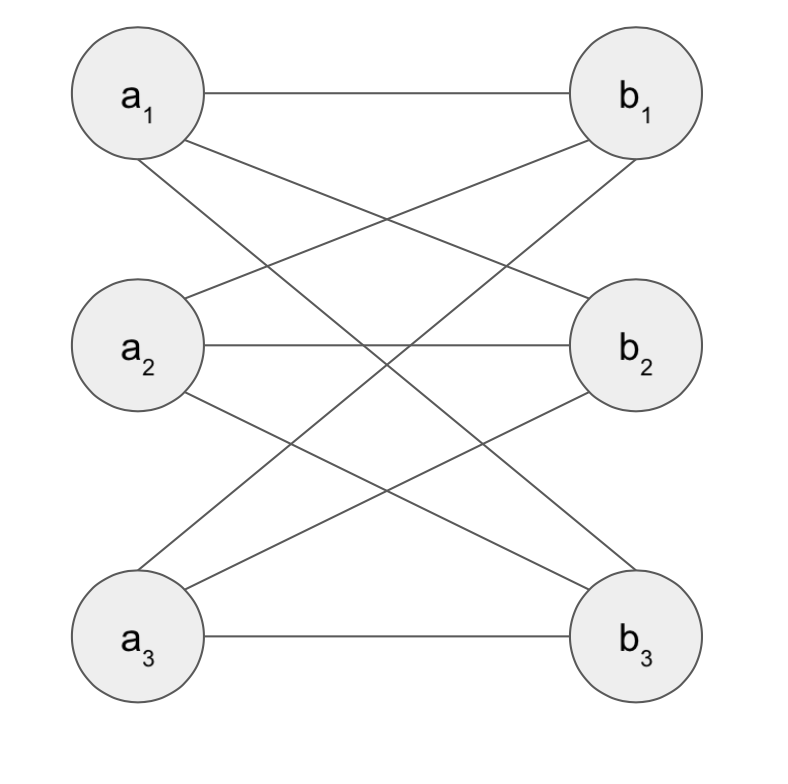
\includegraphics[scale = 0.2]{Bipartite.png}
  \end{center}

  \begin{enumerate}[(a)]
    \item
    How many edges does $B(n)$ have?
    \begin{proof}
      Since each vertex is of degree $n$ and there are $2n$ vertices, $e(B(n)) = n^2$ by the
      Handshake Lemma.
    \end{proof}
    \item
    Let $H(n)$ be the number of Hamiltonian paths of $B(n)$  that start from an $a_i$ vertex and
    ends at a $b_j$ vertex (Hamiltonian paths are paths that go through each vertex exactly once.)
    Prove that $H(n) = (n!)^2$.

    \begin{proof}
      Since $B(n)$ is a complete balanced bipartite graph, we may go from any $a_k$ to any desired
      $b_l$, and vice versa. Hence, counting the number of Hamiltonian paths in $B(n)$ is equivalent
      to counting the orderings of all vertices, where vertices of the same part are adjacent and
      the starting vertex being some $a_i$. Since there the vertices of each part have $n!$
      orderings, $H(n) = (n!)^2$.
    \end{proof}
    
    \item
    Let $P(N)$ be the number of Hamiltonian paths of a Complete Balanced Bipartite Graph on $N$
    vertices. Determine the big-Theta bound of $P(N)$.

    \begin{proof}
      We have already know $P(N) = (\frac{N}{2}!)^2$ when $N$ is even. If $N$ is odd, then
      calculating $P(N)$ is equivalent to calculating $B(n)$ with an additional step of picking out
      a random vertex to be the start. Hence, $P(N) = N(\frac{N - 1}{2}!)^2$ when $N$ is odd.
      Applying Stiring's formula to both cases, we get
      \begin{gather*}
        \left(\frac{N}{2}!\right)^2 \sim \left(\sqrt{\pi N}\left(\frac{N}{2e}\right)^{N - 1/2}\right)^2 = 2^{\log \pi + \log N + N\log N - N\log 2e}
      \end{gather*}
      \begin{align*}
        N\left(\frac{N - 1}{2}!\right)^2 
        &\sim N\left(\sqrt{\pi (N - 1)}\left(\frac{N - 1}{2e}\right)^{N - 1/2}\right)^2 \\
        &= 2^{\log \pi + \log N + \log (N - 1) + (N - 1)\log (N - 1) - (N - 1)\log 2e}.
      \end{align*}
      Hence, in either case, $P(N) = 2^{\Theta(N\log N)} = \Theta(N!)$.
    \end{proof}
  \end{enumerate}
\end{homeworkProblem}

\newpage

\begin{homeworkProblem}
  A {\em triangle}  in an undirected, simple graph is a set of three 
  distinct vertices $x, y, z$ such that all pairs are connected by an edge. 

  \begin{enumerate}[(a)]
  \item
  Consider the following algorithm that takes as input an adjacency matrix of a simple undirected
  graph $G$ and returns True if there exists a triangle and returns False if there is not a
  triangle.

  \begin{quote}
  \emph{Triangle1}$(G)$ ($G$, an undirected simple graph with $n$ vertices in adjacency matrix
  form.)
  \begin{enumerate}[1.]
  \item
  {\bf for} $i = 1,\dots, n$:
  \item
  \ind {\bf for} $j = 1,\dots, n$:
  \item
  \ind \ind {\bf if} $G[i,j] == 1:$
  \item
  \ind\ind\ind {\bf for} $k = 1,\dots, n$:
  \item
  \ind\ind\ind\ind {\bf if} $G[i,k] == 1$ and $G[j,k] == 1$:
  \item
  \ind\ind\ind\ind\ind {\bf return} True
  \item
  {\bf return} False
  \end{enumerate}
  \end{quote}

  Show that the runtime for this algorithm is $O(|V|^2 +|V||E|)$.

  \begin{proof}
    The algorithm finds edges by iterating through pairs of vertices, which takes $O(|V|^2)$ time.
    Upon finding an edge, it proceeds to iterating through vertices to look for the potential vertex
    that completes the triangle, which takes additional $O(|V|)$ time per edge. Hence, the runtime
    for \emph{Triangle1} is $O(|V|^2 + |V||E|)$.

    
  \end{proof}

  \item 
  In order for \emph{Triangle1} to return True, what needs to happen and why does this correspond to
  a triangle?

  \begin{proof}
    \emph{Triangle1} returns true only if it finds an edge between some vertices $u, v$ and there
    exists another vertex $w$ which is adjacent to both $u$ and $v$. In this case, since $u, v, w$
    are pair-wise adjacent, they form a triangle.
  \end{proof}

  \item 
  Consider the following algorithm that takes as input an adjacency matrix of a simple undirected
  graph $G$ and returns True if there exists a triangle and returns False if there is not a
  triangle.

  \begin{quote}
  \emph{Triangle2}$(G)$ ($G$, an undirected simple graph with $n$ vertices in adjacency matrix
  form.)
  \begin{enumerate}[1.]
  \item
  Compute $H = G \times G$.
  \item
  {\bf for} $i = 1,\dots, n$:
  \item
  \ind {\bf for} $j = 1,\dots,n$:
  \item
  \ind\ind {\bf if} $G[i,j] == 1$ AND $H[i,j] > 0$:
  \item
  \ind\ind\ind {\bf return} True
  \item
  {\bf return} False
  \end{enumerate}
  \end{quote}

  
  Assuming that matrix multiplication between two $n\times n$ matrices takes $O(n^{2.81})$ time,
  calculate the runtime of this algorithm. 

  \begin{proof}
    Iterating through pairs of vertices take $O(|V|^2) = O(n^2)$ time. Together with the runtime for
    matrix multiplication, the runtime for this algorithm is $O(n^{2.81} + n^2) = O(n^{2.81})$.
  \end{proof}

  \item
  In order for \emph{Triangle2} to return True, what needs to happen and why does this correspond to
  a triangle? (In particular, what does it mean for $H[i,j] = 1$ or $H[i,j] = 2$?)

  \begin{proof}
    \emph{Triangle2} returns True only when $H[i, j] > 0$ and $G[i, j] == 1$. Note that $H[i, j]$
    records the number of length 2 paths from vertex $i$ to vertex $j$. Hence, $H[i, j] > 0$ and
    $G[i, j] == 1$ indicates that $i, j$ are both adjacent to some vertex $k$ and $i, j$ are also
    adjacent to each other, which makes $i, j, k$ a triangle. 
  \end{proof}

  \item
  Is \emph{Triangle1} or \emph{Triangle2} more efficient? (Justify your answer.) (Hint: think about
  dense and sparse graphs.)

  \begin{proof}
    In dense graphs, $|E|$ is close to $n^2$, which makes the runtime for \emph{Triangle1} around
    $O(n^3)$. But in sparse graphs, $|E|$ far less than $n^2$, which makes the runtime for
    \emph{Triangle1} $O(n^2)$ in this case. Hence, \emph{Triangle1} is more efficient than
    \emph{Triangle2} when $G$ is sparse, and the other way around when $G$ is dense.
  \end{proof}
  \end{enumerate}
\end{homeworkProblem}

\newpage

\begin{homeworkProblem}
  Given a directed graph $G$ with vertex weights $w_v\in\{0,1,2\}$ (in other words, each vertex is
  either labeled with 0, 1 or 2), and vertices $s$ and $t$. Determine if there is a path in $G$ from
  $s$ to $t$ such that the ternary sequence of vertex weights in the path does not repeat the same
  number twice in a row.

  Consider the following algorithm that claims to solve this problem: 

  \begin{quote}
  {\bf Algorithm Description:}

  Input: a $\{0,1,2\}$-labeled directed graph $G$, a vertex $s$ of $G$ and a vertex $t$ of $G$.

  Create a graph $G'$ by removing all edges $(u,v)$ such that $w(u) == w(v)$.

  Run graphsearch on $G'$ starting from $s$. If $t$ is visited then return TRUE. Otherwise return
  FALSE

  \end{quote}

  Prove that this algorithm is correct.

  \begin{proof}
    Suppose there exists a path $P$ from $s$ to $t$ without repeating consecutive numbers, say
    $v_1v_2\ldots v_n$, where $v_1 = s$ and $v_n = t$. Since $w(v_i) \neq w(v_{i + 1})$ for all $i$,
    all edges of $P$ remains in $G'$, and thus $P \subseteq G'$. It follows that $t$ can be visited
    from $s$ with graphsearch on $G'$ via $P$, so the algorithm returns TRUE.

    Suppose not. We may assume there exists a path $P$ from $s$ to $t$ in $G$, otherwise $t$ is also
    not reachable from $s$ in $G' \subseteq G$ and we are done. Then, $P$ must include some edge
    $(v_i, v_{i + 1})$ such that $w(v_i) = w(v_{i + 1})$. But then $(v_i, v_{i + 1}) \notin E(G)$,
    so any paths from $s$ to $t$ in $G$ do not remain in $G'$, and thus the algorithm return FALSE.

    Therefore, the algorithm is correct.
  \end{proof}
\end{homeworkProblem}
\end{document}